\documentclass[11pt,a4paper,oldfontcommands,oneside]{memoir}
\usepackage[utf8]{inputenc}
\usepackage{microtype}
\usepackage[dvips]{graphicx}
\usepackage{xcolor}
\usepackage{times}
\usepackage{graphicx}
\usepackage[spanish]{babel}
\usepackage[
breaklinks=true,colorlinks=true,
%linkcolor=blue,urlcolor=blue,citecolor=blue,% PDF VIEW
linkcolor=black,urlcolor=black,citecolor=black,% PRINT
bookmarks=true,bookmarksopenlevel=2]{hyperref}

\usepackage{geometry}
% PDF VIEW
% \geometry{total={210mm,297mm},
% left=25mm,right=25mm,%
% bindingoffset=0mm, top=25mm,bottom=25mm}
% PRINT
\geometry{total={210mm,297mm},
left=20mm,right=20mm,
bindingoffset=10mm, top=25mm,bottom=25mm}

\OnehalfSpacing
%\linespread{1.3}

%%% CHAPTER'S STYLE
\chapterstyle{bianchi}
%\chapterstyle{ger}
%\chapterstyle{madsen}
%\chapterstyle{ell}
%%% STYLE OF SECTIONS, SUBSECTIONS, AND SUBSUBSECTIONS
\setsecheadstyle{\Large\bfseries\sffamily\raggedright}
\setsubsecheadstyle{\large\bfseries\sffamily\raggedright}
\setsubsubsecheadstyle{\bfseries\sffamily\raggedright}


%%% STYLE OF PAGES NUMBERING
%\pagestyle{companion}\nouppercaseheads 
%\pagestyle{headings}
%\pagestyle{Ruled}
\pagestyle{plain}
\makepagestyle{plain}
\makeevenfoot{plain}{\thepage}{}{}
\makeoddfoot{plain}{}{}{\thepage}
\makeevenhead{plain}{}{}{}
\makeoddhead{plain}{}{}{}


\maxsecnumdepth{subsection} % chapters, sections, and subsections are numbered
\maxtocdepth{subsection} % chapters, sections, and subsections are in the Table of Contents


%%%---%%%---%%%---%%%---%%%---%%%---%%%---%%%---%%%---%%%---%%%---%%%---%%%

\begin{document}

%%%---%%%---%%%---%%%---%%%---%%%---%%%---%%%---%%%---%%%---%%%---%%%---%%%
%   TITLEPAGE
%
%   due to variety of titlepage schemes it is probably better to make titlepage manually
%
%%%---%%%---%%%---%%%---%%%---%%%---%%%---%%%---%%%---%%%---%%%---%%%---%%%
\thispagestyle{empty}

{%%%
\sffamily
\centering
\Large

~\vspace{\fill}

\includegraphics[scale=1]{logo.png} \\
{\huge 
\vspace{4cm}
Explicar el Operador Jacobiano
}
\vspace{2.5cm}

{\LARGE
Eduardo Robles Vázquez
}

\vspace{2.5cm}

Universidad Politécnica de la Zona Metropolitana de Guadalajara

\vspace{3.5cm}

Profesor: Carlos Enrique Morán Garabito

\vspace{\fill}

15 de Octubre de 2019

%%%
}%%%

\vspace{.5cm}
\hfill\break
\tableofcontents*
\clearpage

%%%---%%%---%%%---%%%---%%%---%%%---%%%---%%%---%%%---%%%---%%%---%%%---%%%
%%%---%%%---%%%---%%%---%%%---%%%---%%%---%%%---%%%---%%%---%%%---%%%---%%%
\chapter{Operador Jacobiano}
La matriz Jacobiana es una matriz formada por las derivadas parciales de primer orden de una función. Una de las aplicaciones más interesantes de esta matriz es la posibilidad de aproximar linealmente a la función en un punto. En este sentido, el jacobiano representa la derivada de una función multivariable. Propiamente deberíamos hablar más que de matriz jacobiana, de diferencial jacobiana o aplicación lineal jacobiana ya que la forma de la matriz dependerá de la base o coordenadas elegidas. Es decir, dadas dos bases diferentes la aplicación lineal jacobiana tendrá componentes diferentes aun tratándose del mismo objeto matemático. La propiedad básica de la "matriz" jacobiana es la siguiente, dada una aplicación cualquiera:

\begin{center}
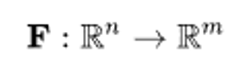
\includegraphics[scale=.75]{1.png} \\
\end{center}
 
Continua, es decir: \\

\begin{center}
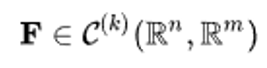
\includegraphics[scale=.75]{2.png} \\
\end{center}

Se dirá que es diferenciable si existe una aplicación lineal: \\

\begin{center}
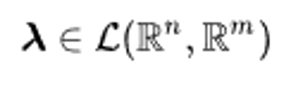
\includegraphics[scale=.75]{3.png} \\
\end{center}

Tal que: \\

\begin{center}
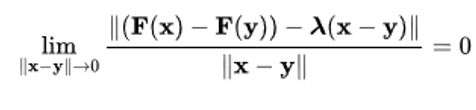
\includegraphics[scale=.75]{4.png} \\ 
\end{center}

\section{Función escalar}
Empecemos con el caso más sencillo de una función escalar: \\

\begin{center}
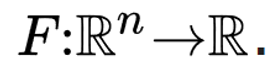
\includegraphics[scale=.5]{5.png} \\
\end{center}

En este caso la matriz jacobiana será una matriz formada por un vector fila que coincide con el gradiente. Si la función admite derivadas parciales para cada variable puede verse que basta definir la "matriz" jacobiana como: \\

\begin{center}
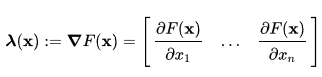
\includegraphics[scale=1]{6.png} \\
\end{center}
 
Ya que entonces se cumplirá la relación automáticamente, por lo que en este caso la "matriz jacobiana" es precisamente el gradiente. 

\section{Función vectorial}
Supongamos:

\begin{center}
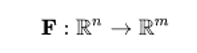
\includegraphics[scale=1]{7.png}  
\end{center}

Es una función que va del espacio euclídeo n-dimensional a otro espacio euclídeo m-dimensional. Esta función está determinada por m funciones escalares reales:

\begin{center}
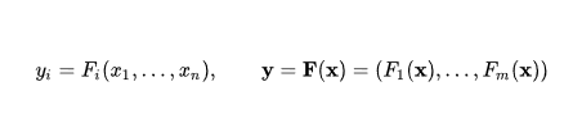
\includegraphics[scale=1]{8.png} 
\end{center}

Cuando la función anterior es diferenciable, entonces las derivadas parciales de estas m funciones pueden ser organizadas en una matriz m por n, la matriz jacobiana de F: \\

\begin{center}
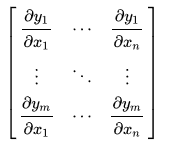
\includegraphics[scale=1]{9.png} 
\end{center}

Esta matriz es notada de diversas maneras:

\begin{flushleft}
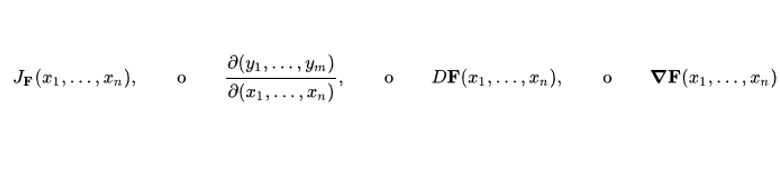
\includegraphics[scale=.85]{10.png}
\end{flushleft}


Nótese que la fila, i-ésima fila coincidirá dada con el gradiente de la función $Y_i$, para $i = 1,...,m$. Si $p$ es un punto de $R_n$ y $F$ es diferenciable en $p$, entonces su derivada está dada por $J_F (p)$. En este caso, la aplicación lineal descrita por $J_F (p)$ es la mejor aproximación lineal de $F$ cerca del punto $p$, de esta manera:

\begin{center}
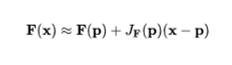
\includegraphics[scale=1.25]{11.png}
\end{center}

Para $x$ cerca de $p$. O con mayor precisión:

\begin{center}
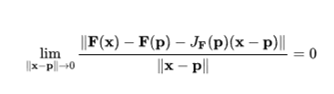
\includegraphics[scale=1.25]{12.png} \\
\end{center}

\vspace{2cm}
\hfill
\bibliographystyle{unsrt}

\bibliography{biblio}
\end{document}


\end{document}

